\documentclass[11pt]{article}
\usepackage[a4paper,margin=2.4cm]{geometry}
\usepackage{graphicx}
\usepackage{booktabs}
\usepackage{xcolor}
\usepackage{titlesec}
\usepackage{parskip}
\usepackage[hidelinks]{hyperref}
\titleformat{\section}{\large\bfseries\color{black!80}}{\thesection}{0.6em}{}
\titleformat{\subsection}{\normalsize\bfseries}{\thesubsection}{0.5em}{}
% caption-safe monospace path (handles underscores in moving arguments)
\DeclareRobustCommand{\fpath}[1]{{\small\texttt{\detokenize{#1}}}}

\title{\vspace{-1.2cm}\textbf{Storyline outline --- zonality of soil-carbon turnover}\\[2pt]
\large Working document for comment (not the manuscript)}
\author{}
\date{2026-06-26}

\begin{document}
\maketitle
\vspace{-0.8cm}

\noindent\textit{This is the operational story bible: the narrative bones, the four
pillars, the figures we plan to use (with comments), and the key numbers --- all
backed by repeatable scripts. Numbers are the production values (500-tree models,
MAIN 6-layer biology) unless noted. Its companion is}
\fpath{results_reconciliation_2026-06-26.md} \textit{(number map, figure
dispositions, manuscript checklist). Read this; then we write the manuscript
together.}

% =============================================================================
\section{Thesis and contribution}

\textbf{One sentence.} Beyond climate, soil-carbon turnover carries a coherent,
attributable, and mappable spatial organisation --- modest in magnitude but real
--- that Earth System Models (ESMs) over-represent and disagree on; we offer it
both as an interpretive framework and as an observational benchmark.

That climate does not fully control soil carbon is not new (Schmidt et al.\ 2011
made the case a decade ago). \emph{Our} contribution is not the \emph{existence}
of a beyond-climate signal but its \emph{organisation}: we show the residual is
spatially structured rather than noise, we attribute it to mechanistic process
classes in an order-independent way, and we map where it acts. The framing is
deliberately tool-first --- a way of \emph{reading} non-climate turnover
structure --- with the ESM contrast as the closing ``so what'', rather than a
paper whose entire weight rests on a model critique.

A second, honest pillar of the contribution is restraint. The beyond-climate
signal is real but small ($\sim$7 percentage points of explained variance), most
of the point-scale residual is unstructured noise, and the organised part only
emerges at coarse (meso) scale. We treat this modesty as a feature: every claim
is made on a spatially-honest footing and survives a battery of robustness checks.

% =============================================================================
\section{Narrative spine (OCAR)}

\textbf{Opening.} Soil-carbon turnover is routinely treated as climate-driven,
with the remainder dismissed as noise or left unresolved. Yet on a
\emph{spatially-honest} basis --- block cross-validation that prevents nearby
samples from leaking between training and test --- climate explains only about
\emph{one third} of the predictable variance in turnover time.

\textbf{Challenge.} Is the other two thirds merely noise, or is it (i)
spatially \emph{organised}, (ii) \emph{attributable} to identifiable process
classes, and (iii) \emph{mappable}? And if it is organised, do the ESMs we rely
on for projections represent that organisation correctly?

\textbf{Action.} We answer with four complementary analyses on one common
dataset --- an order-independent variance attribution (Shapley), a test of
spatial organisation (Moran's $I$), a meso-scale zonality map, and mechanistic
response curves (ALE) --- each wrapped in an honesty apparatus (spatial
block-CV, a noise-floor analysis, a provenance control, a biological-parsimony
check, and a block-size sensitivity).

\textbf{Resolution.} The beyond-climate signal is a coherent,
ecologically-interpretable zonality: edaphic-led, with soil biology forming a
distinct second axis. It is modest in size but spatially organised and
ecological in origin (not a sampling artifact). ESMs amplify it far too steeply
toward the poles ($\sim$3.6$\times$ on average) and disagree among themselves by
an order of magnitude. We deliver the pattern as a framework for interpretation
and a benchmark for models.

% =============================================================================
\section{The four pillars}

Each pillar answers a distinct question and has a dedicated figure. Together they
make framing A concrete: \emph{how much} (attribution), \emph{where} (map),
\emph{how} (mechanism), and \emph{so what} (ESM contrast).

\subsection{Attribution --- ``how much?'' (Shapley)}

We fit nested Random Forests on a \emph{single common row set} (so coalition
$R^2$ are mutually comparable) and decompose the spatially cross-validated
predictable variance with Shapley values, which average each domain's
contribution over all orderings and therefore avoid the arbitrariness of nested
increments. The split is Climate~35\%, Edaphic~33\%, Biological~22\%,
LandUse~10\% --- i.e.\ climate is only about a third, and non-climate domains
carry two thirds. Strikingly, edaphic properties predict turnover \emph{as well
as climate does on their own} (single-domain $R^2$ tie at 0.31). The single
domains sum to far more than the full model ($0.95$ vs $0.38$), a large overlap
of $0.57$: the domains are \emph{correlated, not redundant}. This is the
conceptual keystone --- it is why a per-pixel ``which-process-wins-here'' map
fails (the channels are too correlated to argmax) while the aggregate attribution
succeeds.

\begin{figure}[h!]\centering
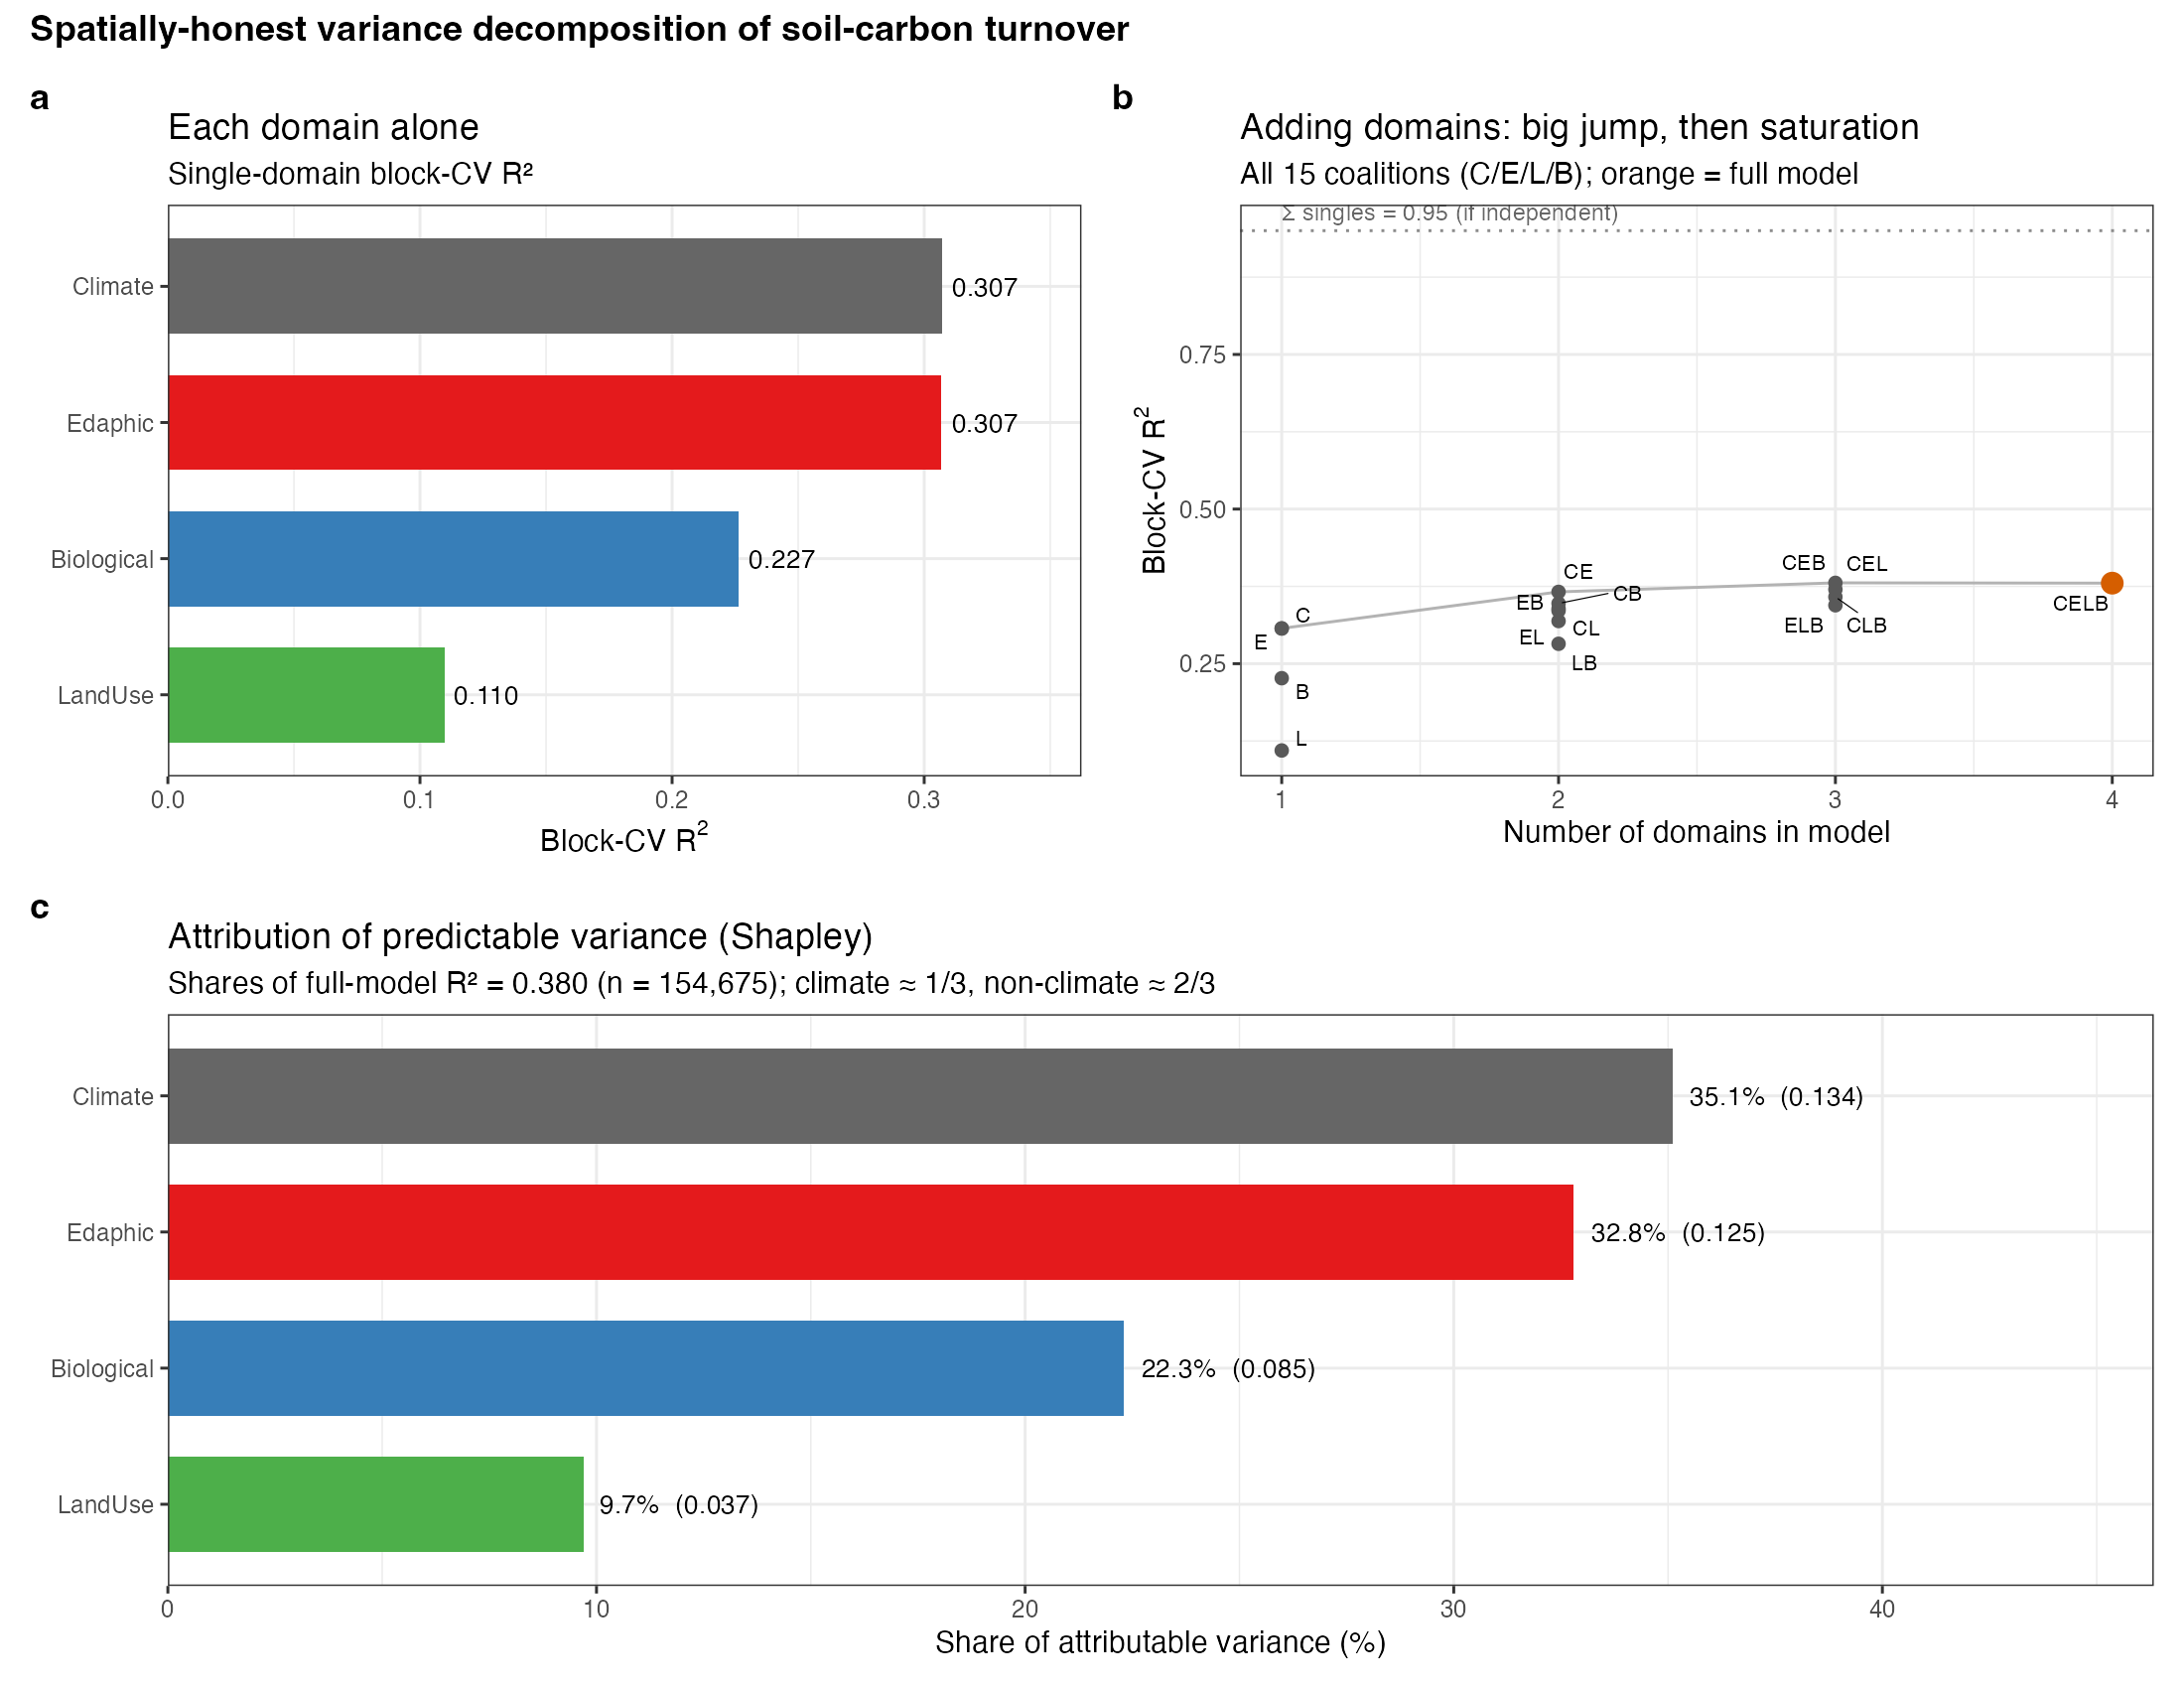
\includegraphics[width=0.96\textwidth]{../../plots/step_13c_commonality/13c_decomposition.png}
\caption{\textbf{Variance decomposition (Results).} Singles $\to$ build-up across
coalitions $\to$ Shapley shares. The build-up panel makes the overlap visible
(the full model sits far below the sum-of-singles line). \fpath{13c_results_figure.R}}
\end{figure}

\subsection{Zonality map --- ``where?''}

We map the log-ratio of nested model predictions --- how much non-climate context
bends predicted turnover relative to a simpler model --- at meso (2\textdegree)
scale, because the residual is two-thirds noise at the native pixel. The
\emph{symmetric} formulation (each domain taken relative to climate; no
abiotic-before-biology ordering) is the main figure, consistent with the
order-independent Shapley attribution. The abiotic panel is near-global over
soil-bearing land and shows a coherent geography: non-climate context
\emph{lengthens} turnover in the Amazon and Congo basins (deep, weathered,
low-fertility clays that stabilise carbon) and \emph{shortens} it across drylands
(Sahel margins, central Asia, Australia). This is the pattern that earns the word
``zonality.''

\begin{figure}[h!]\centering
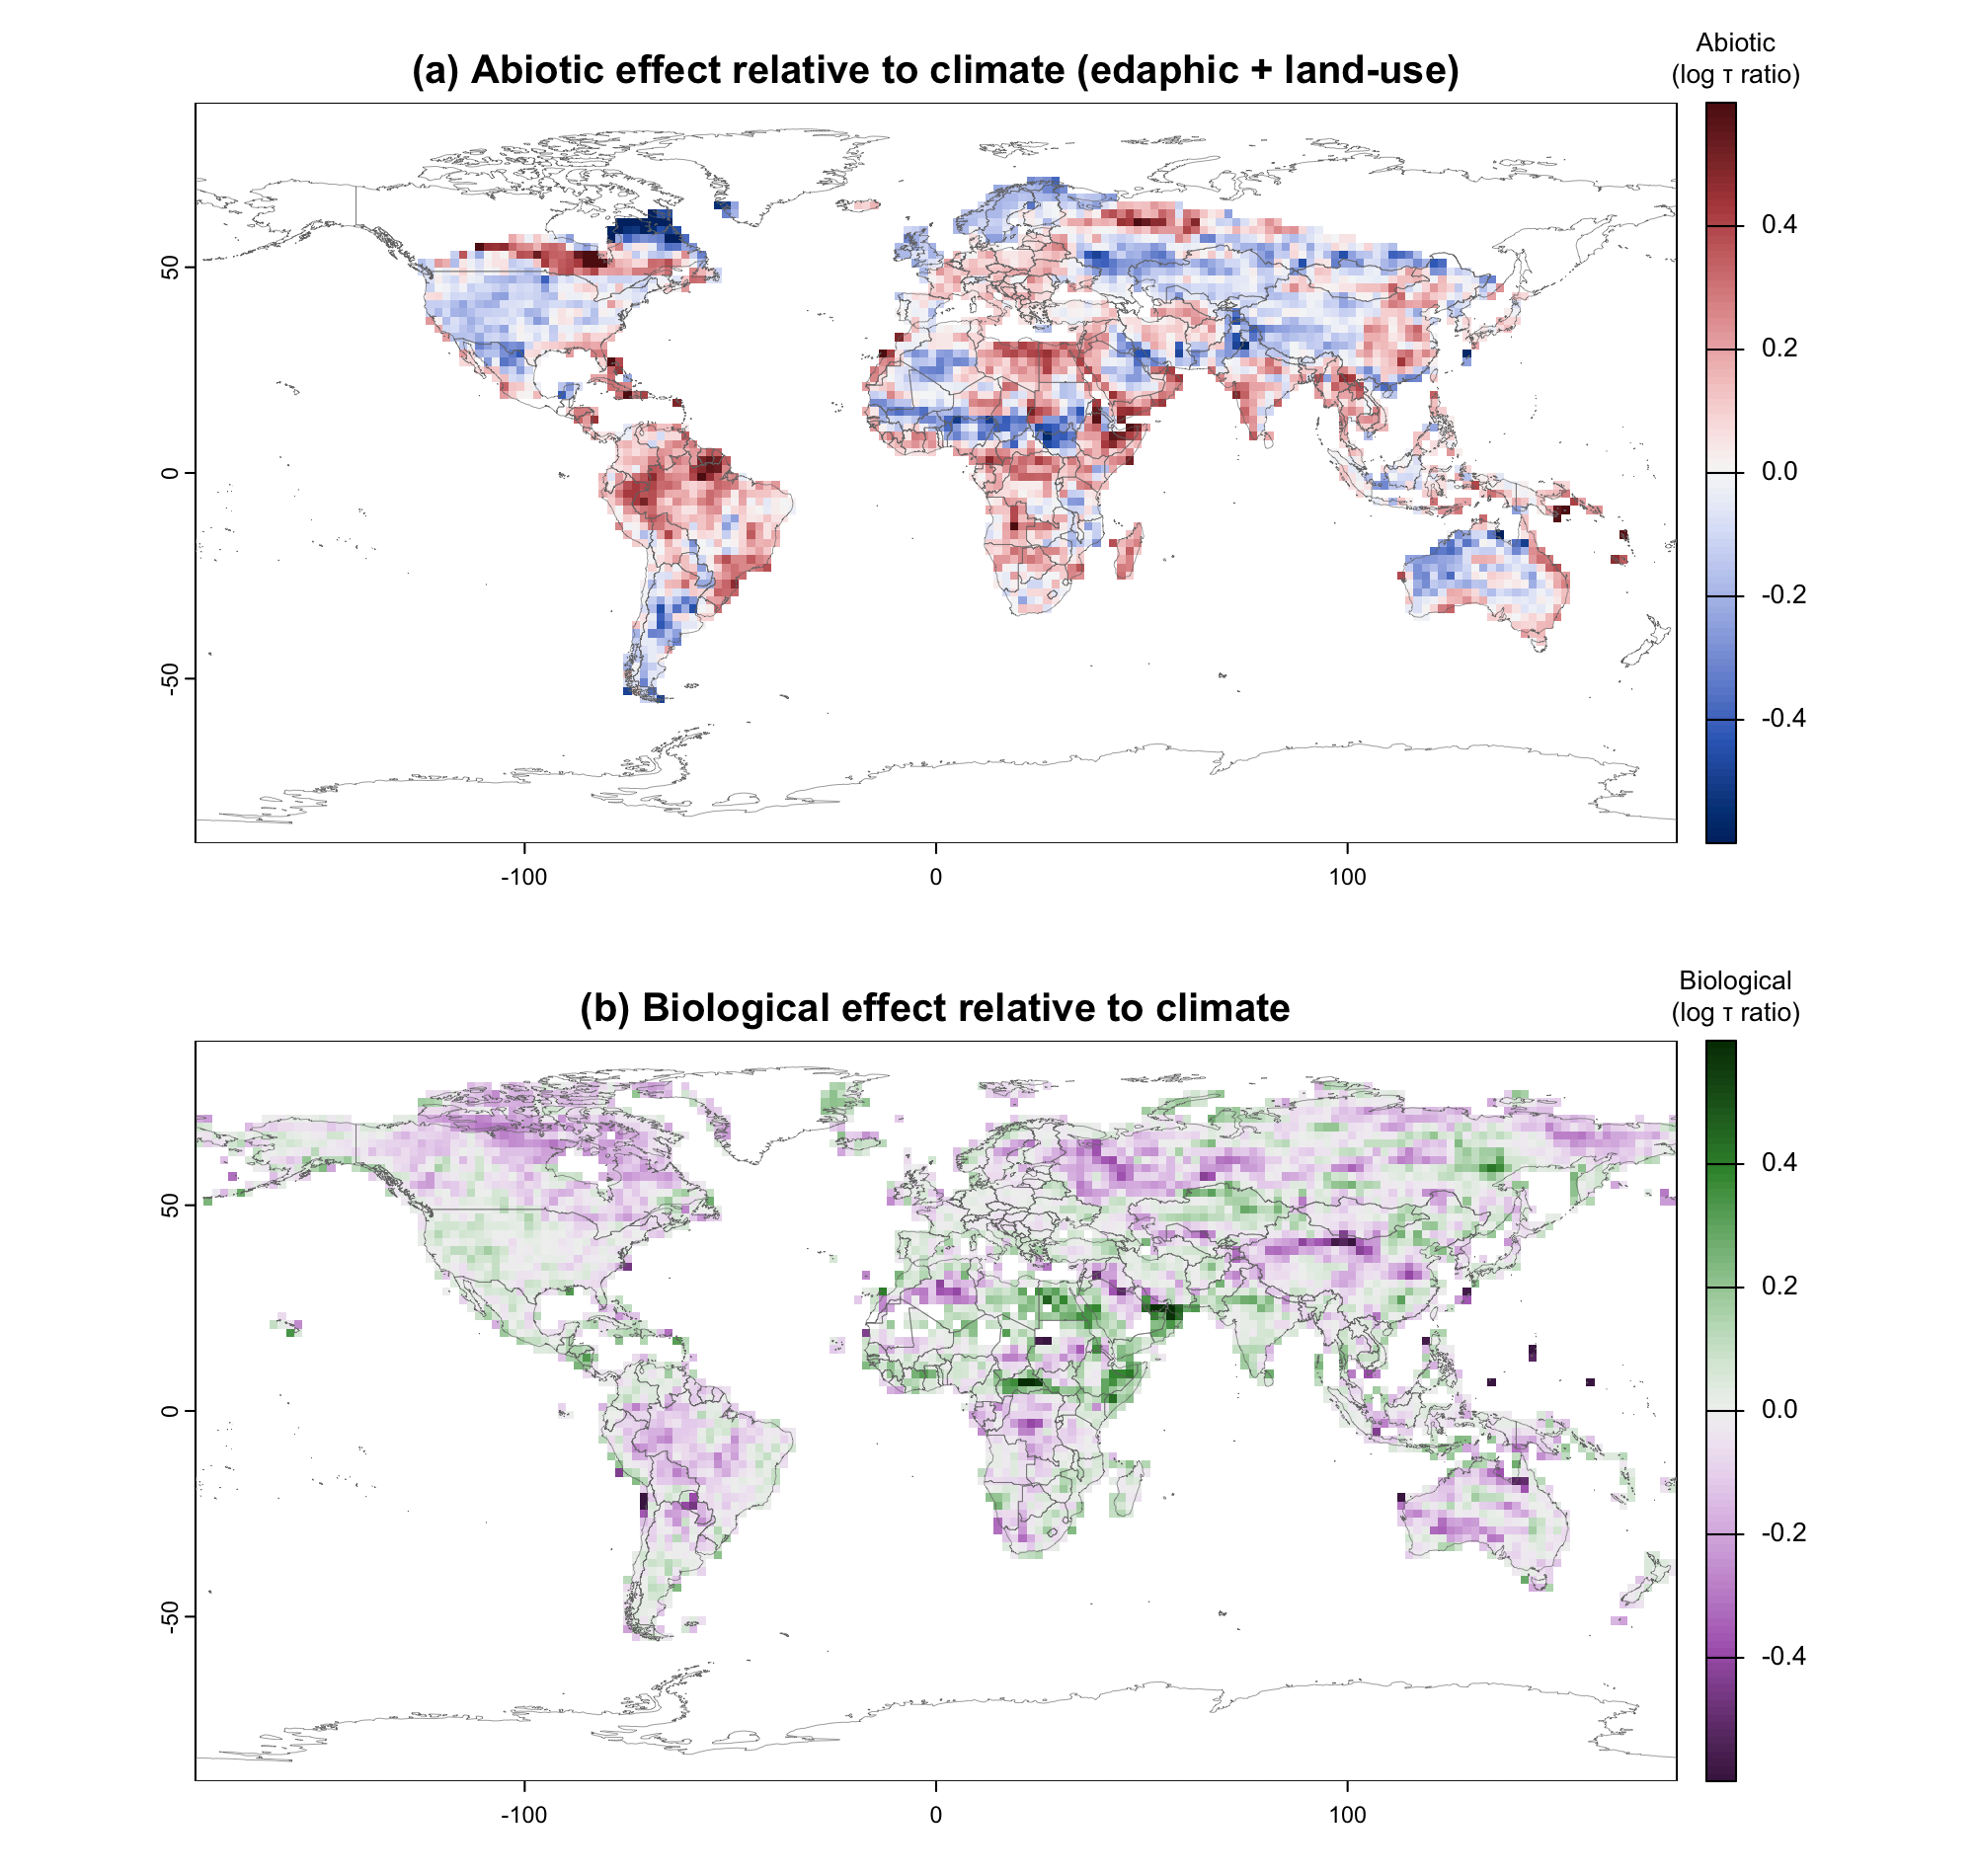
\includegraphics[width=0.82\textwidth]{../../plots/step_15b_zonality/zonality_map_dual_symmetric.png}
\caption{\textbf{Zonality map, symmetric (Results).} (a) Abiotic and (b)
biological modulation, each relative to climate. Red/green = longer turnover,
blue/purple = shorter. The abiotic panel doubles as the near-global headline. The
nested formulation and the abiotic-vs-biology scatter are appendix figures.
\fpath{15b_zonality_map.R}}
\end{figure}

\subsection{Mechanism --- ``how?'' (ALE)}

Accumulated Local Effects give the marginal, functional response of turnover to
each predictor. The curves are clean and mechanistically sensible: turnover
increases with temperature seasonality, snow cover, and elevation; decreases with
sand fraction, bulk density, and soil temperature; and is humped in pH. This is
the layer that turns the attribution and the map into \emph{mechanism} --- it
says not just that edaphic matters and where, but \emph{how} each property acts.

\begin{figure}[h!]\centering
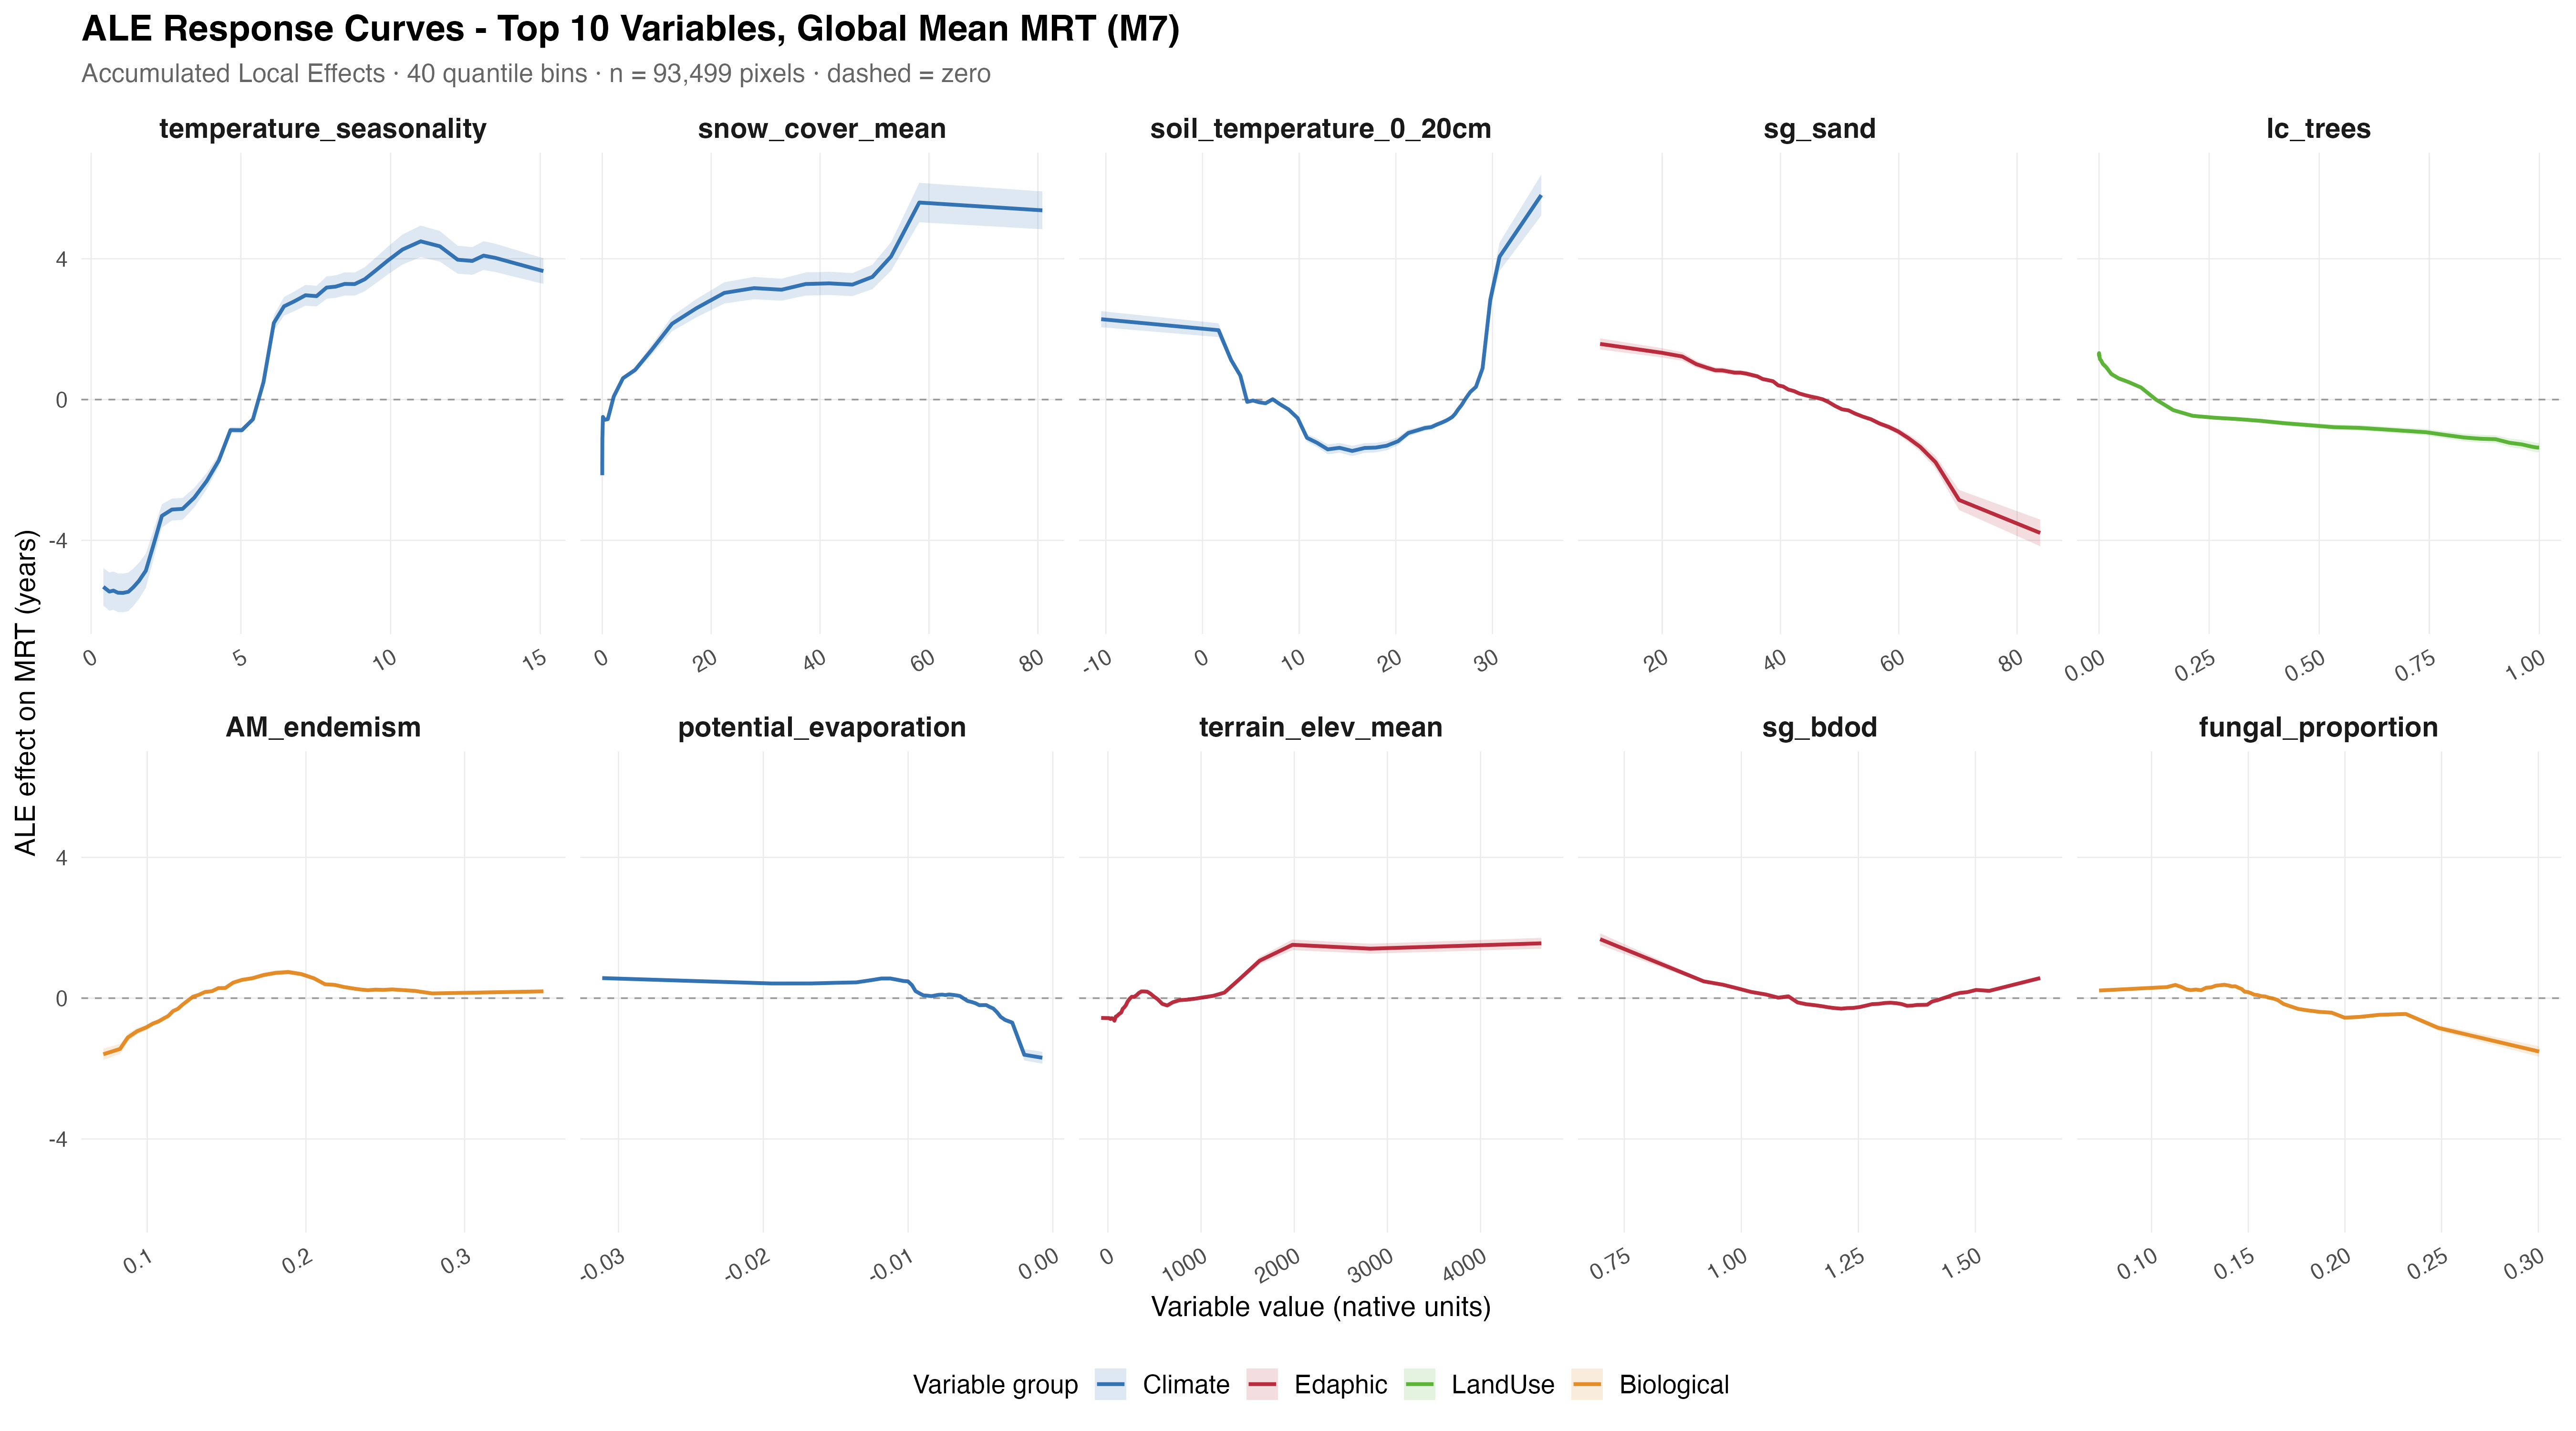
\includegraphics[width=0.96\textwidth]{../../plots/step_18_sensitivity/18D_ALE_top10_MRT.png}
\caption{\textbf{ALE response curves (Results).} Top-10 predictors, coloured by
domain. \fpath{18_sensitivity_analysis.R}}
\end{figure}

\subsection{ESM contrast --- ``so what?''}

We compare the spatial \emph{structure} of turnover against six structurally
independent CMIP6 models. Absolute turnover times are not comparable across
products (depth, pool, and reference-period definitions differ), so we normalise
each product to its own global mean and compare structure --- a choice that
pre-empts the ``apples to pears'' critique. The result is sharp: observations
show a gentle zonality (polar turnover $\sim$2.5$\times$ tropical), whereas the
ESM ensemble amplifies it $\sim$5$\times$ (individual models up to $\sim$14$\times$),
and the models disagree among themselves across an order of magnitude --- one
(MPI) even inverts the gradient. The over-zonalization factor (ensemble vs
observations) is $\sim$3.6$\times$.

\begin{figure}[h!]\centering
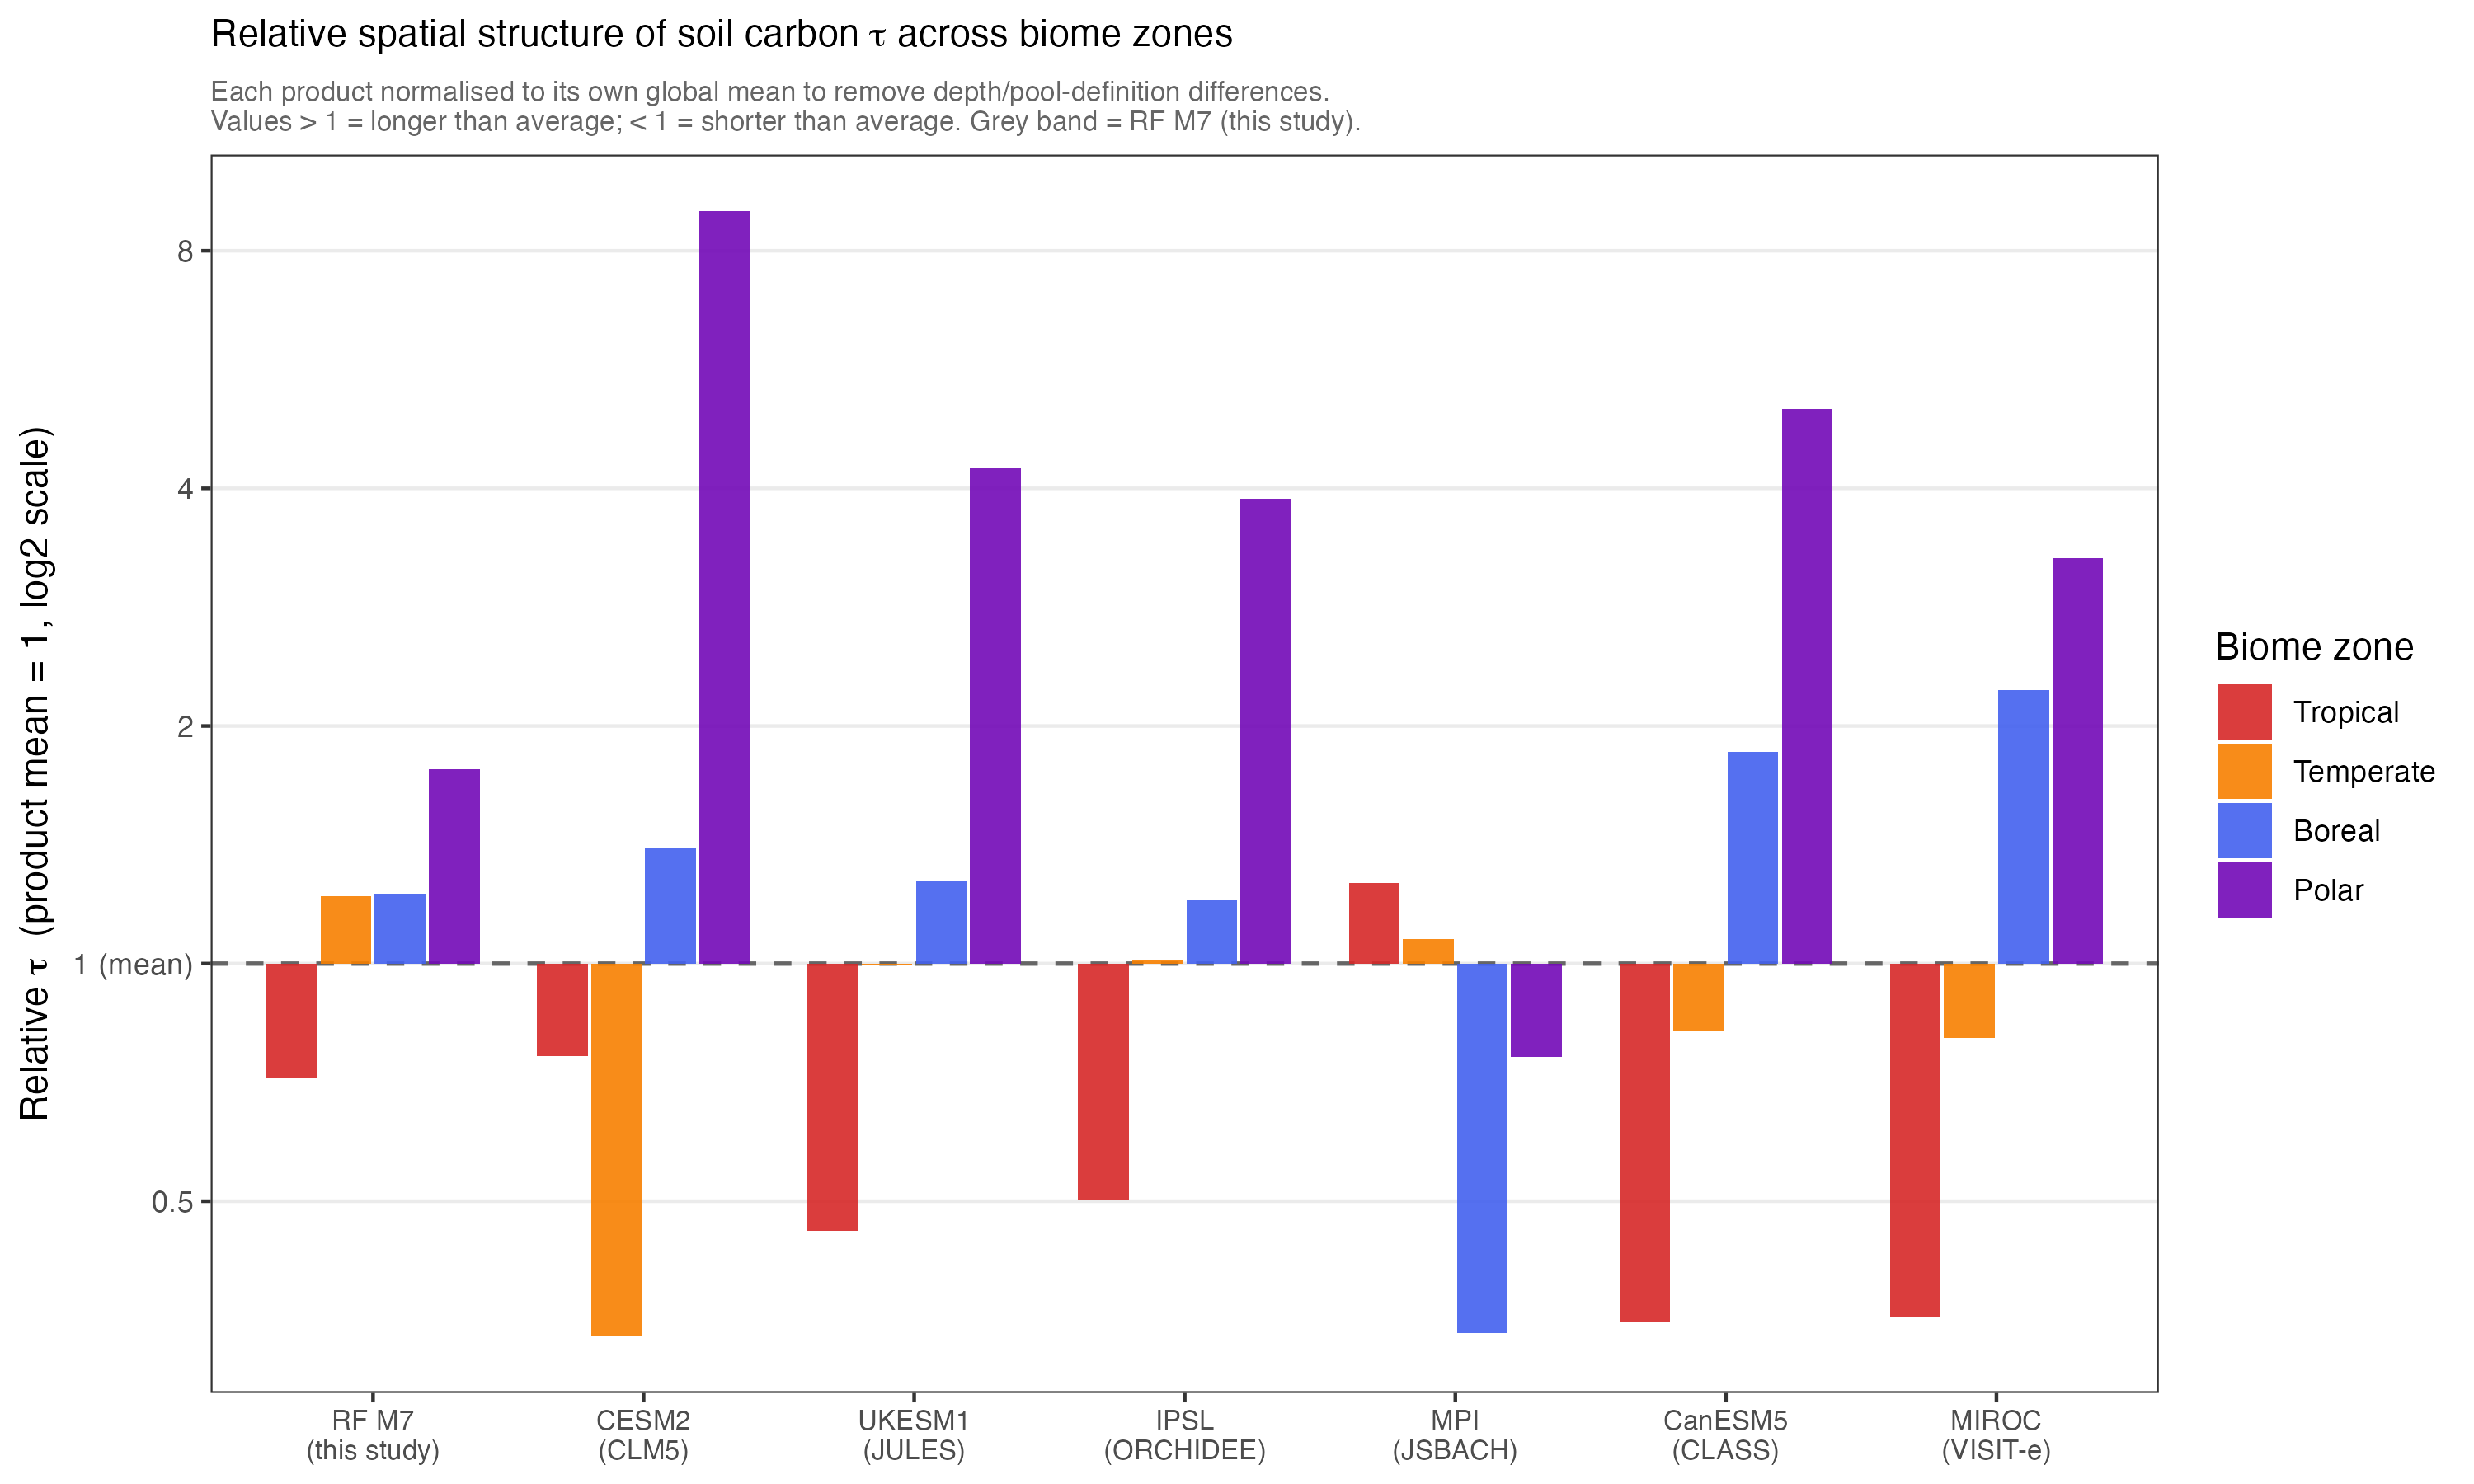
\includegraphics[width=0.96\textwidth]{../../plots/step_20/fig_biome_relative_tau.png}
\caption{\textbf{ESM structural comparison (Results).} Relative turnover by biome
zone, each product normalised to its own global mean. \fpath{20_CMIP_comparison.R};
amplification ratios \fpath{20b_zonal_amplification.R}}
\end{figure}

% =============================================================================
\section{The honesty apparatus (robustness; mostly appendix)}

These analyses do not carry the argument but they make the modest signal
trustworthy. Each is a numbered, repeatable script.

\textbf{Spatial block cross-validation.} All skill is estimated by holding out
whole 2\textdegree{} blocks, so reported $R^2$ is a true out-of-region
generalisation number, not interpolation between near-neighbours.

\textbf{Noise floor.} The residual variogram has a nugget/sill of $\sim$0.56 and a
range of $\sim$16~km: roughly two thirds of the beyond-climate residual is
unstructured noise, and structure lives only at short range. This is why we map
at meso scale and never show native-pixel texture.

\textbf{Provenance control.} Only 2.4\% of the residual variance lies between the
44 source databases; removing each source's mean barely changes the coarse
organisation or covariate skill. The signal is ecological, not a
laboratory/compilation artifact. (Conservative, since source is confounded with
geography.)

\textbf{Biological parsimony.} The biological signal is multidimensional, but the
three Barcel\'o root-colonisation layers are statistically inert ($+0.001$ unique
$R^2$) while capping coverage. Dropping them lifts the biological footprint from
61\% to 96\% of sampled rows with no loss of skill; the full nine-layer set is
kept as a sensitivity case.

\textbf{Block-size invariance.} Re-running the decomposition with 1\textdegree{}
and 5\textdegree{} blocks moves each Shapley share by at most 2.4 percentage
points, even though absolute $R^2$ declines with block size --- attribution is
robust to the scale choice.

\textbf{Spatial correlation of the two axes.} Abiotic and biological modulation
co-vary when each is taken over climate ($r\approx0.4$--$0.5$) but are orthogonal
once biology is taken conditional on the abiotic model ($r\approx0$). This is the
overlap/``correlated, not redundant'' result expressed spatially, and it is its
own appendix scatter figure (Köppen-coloured).

% =============================================================================
\section{Key numbers}

\begin{table}[h!]\centering\small
\begin{tabular}{ll}
\toprule
Quantity & Value \\
\midrule
Full-model block-CV $R^2$ & 0.38 (climate alone 0.31; beyond-climate $\sim$7~pp) \\
Shapley shares (C/E/B/L) & 35 / 33 / 22 / 10 \% \\
Single-domain $R^2$ & C 0.31 $\approx$ E 0.31 $>$ B 0.23 $\gg$ L 0.11 \\
Overlap ($\Sigma$ singles $-$ full) & 0.57 (correlated, not redundant) \\
Tier-1 organisation (Moran's $I$) & 0.25 ($p\ll0.001$) \\
Noise floor (nugget/sill; range) & 0.56; $\sim$16~km \\
Between-source variance share & 2.4\% (ecological, not provenance) \\
Block-size invariance & shares move $\le$2.4~pp over 1--5\textdegree \\
Biological coverage (MAIN set) & 96\% of rows (vs 61\% with Barcel\'o) \\
Over-zonalization (ESM vs obs) & polar/tropical 2.5$\times$ vs $\sim$9$\times$; factor $\sim$3.6$\times$ \\
\bottomrule
\end{tabular}
\end{table}

% =============================================================================
\section{Figure plan}

\begin{table}[h!]\centering\small
\begin{tabular}{lll}
\toprule
Figure & Destination & Comment \\
\midrule
Zonality map (symmetric) & Results & where; abiotic panel = near-global headline \\
Variance decomposition & Results & how much + the overlap keystone \\
ALE response curves & Results & how each driver acts (mechanism) \\
ESM biome-relative & Results & so what; structural over-zonalization \\
Tier-1 residual map + Moran & Results/App. & organisation is real, not noise \\
Scale / noise-floor & Appendix & two-thirds noise; meso-scale justification \\
Provenance table & Appendix & ecological, not artifact \\
Block-size sensitivity & Methods & justifies 2\textdegree{} choice \\
Biological parsimony & Appendix & why drop Barcel\'o; keep 9 as sensitivity \\
Nested map + abiotic/biology scatter & Appendix & order-dependence; correlated-not-redundant \\
Relative latitude heatmap & Appendix & continuous-latitude ESM structure \\
Absolute latitudinal profile & Appendix & the resolved-tension side-arc (below) \\
Sampling coverage & Methods/Data & where/when sampled \\
\midrule
\textit{Dropped (obsolete)} & --- & step-17 M1--M7 maps, all-models comparison, \\
 & & latitude histogram; step-20 absolute heatmap \\
\bottomrule
\end{tabular}
\end{table}

% =============================================================================
\section{Two deliberate narrative devices}

\textbf{Own the incomparability.} In the ESM section we state up front that
absolute turnover is not comparable across products, and therefore compare only
normalised spatial structure. Declaring the limitation first, and controlling for
it, converts a potential ``apples to pears'' objection into a deliberate,
rigorous design choice.

\textbf{Resolved-tension side-arc (Discussion).} We briefly raise the
absolute-magnitude caveat (with the absolute latitudinal profile relegated to the
appendix) and then resolve it via the structural comparison. It is a small arc
for robustness, signalling that we considered and dismissed the obvious
objection; it is not central to the argument.

% =============================================================================
\section{Status and next steps}

\textbf{Settled.} Shapley-primary lead; tool-first framing; symmetric map as the
Results centerpiece with the nested version and the scatter in the appendix; the
abiotic-vs-biology correlation reported briefly in the Discussion; the ESM
section reframed as structural; step-17 demoted, step-18 kept, step-20's absolute
profile moved to the appendix side-arc.

\textbf{Open (small).} A minimum-fill coverage threshold for the meso maps; an
optional per-pixel Shapley map as the order-free gold standard (needs a step-14
extension); and a final refresh of the (currently 300-tree) block-size sweep at
500 trees.

\textbf{Consistency item for the post-freeze code polish.} The ALE (step~18) and
the prediction maps (step~14) were built on the all-nine-layer biology model;
for full consistency the final pass should regenerate them with the MAIN 6-layer
set. This does not affect the climate/edaphic curves or the abiotic map, so it is
cleanup, not a story risk.

\textbf{Next.} The prose pass: draft \fpath{manuscript.tex} section by section
against this outline and the reconciliation memo, then a code-polish pass once the
story is frozen.

\end{document}
